% 2013 年安徽卷理科第 19 题：圆锥 P-O，底面圆 O 上的两条平行弦 AB、CD。
% 来源 PDF：普通高考/2013/2013安徽理.pdf，第 2 页（印面 784）左栏。
% AB 与 CD 均为底面圆的弦且 AB ∥ CD；O 为底面圆心，OP 为轴。
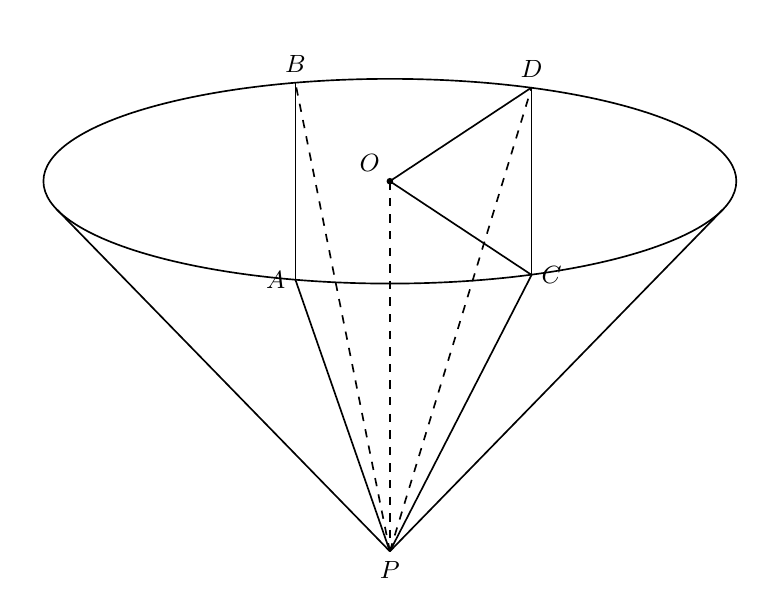
\begin{tikzpicture}[semithick, font=\small]
  \useasboundingbox (-4.6,-5.15) rectangle (4.6,1.95);
  \coordinate (O) at (0,0);
  \coordinate (A) at (-1.2,-1.25);
  \coordinate (B) at (-1.2,1.25);
  \coordinate (C) at (1.8,-1.19);
  \coordinate (D) at (1.8,1.19);
  \coordinate (P) at (0,-4.7);
  % 底面圆（椭圆示意）
  \draw (O) ellipse [x radius=4.4, y radius=1.3];
  % 两条平行弦
  \draw (A) -- (B);
  \draw (C) -- (D);
  % 圆心与轴
  \draw[dashed] (O) -- (P);
  \fill (O) circle (1.2pt);
  % 半径 OC、OD
  \draw (O) -- (C);
  \draw (O) -- (D);
  % 轮廓母线（P 向椭圆的切线）为实线；P-A、P-C 在前方为实线，P-B、P-D 被遮挡为虚线
  \coordinate (L) at (-4.228,-0.360);
  \coordinate (R) at (4.228,-0.360);
  \draw (P) -- (L);
  \draw (P) -- (R);
  \draw (P) -- (A);
  \draw (P) -- (C);
  \draw[dashed] (P) -- (B);
  \draw[dashed] (P) -- (D);
  % 标注
  \node[above left] at (O) {$O$};
  \node[left] at (A) {$A$};
  \node[above] at (B) {$B$};
  \node[right] at (C) {$C$};
  \node[above] at (D) {$D$};
  \node[below] at (P) {$P$};
\end{tikzpicture}
